\chapter{Results and Discussion}

\section{Pipeline}
\subsection{Input}
\subsection{Distances}
\subsection{Structure Realization}
\subsection{Evaluation and Visualization}

\begin{itemize}
    \item TM score, GDT\_TS
\end{itemize}
    
\section{Distance predictions}
\subsection{Perceptron}
\subsection{Simple CNN (LeNet)}
\subsection{AlphaFold}
\subsection{Overtraining of the model}
We performed an experiment, to observe how our model behaves with different kinds of data.
First, we initialized the model parameters randomly.
Our primary expectation was that, if we use also randomly generated input and no training, the output will look very randomly as well.
% This expectation is visualized in the Figure (\ref{fig:in_out_dep1}).
    
% \begin{figure}
%     \centering
%     \includegraphics{}
%     \caption{Caption}
%     \label{fig:in_out_dep1}
% \end{figure}
    
Surprisingly, this was not the case in the experiment.
    
\begin{itemize}
    \item Architecture (Blocks, dilated convolutions, groups)
    \item Number of parameters
    \item Projections (Up, Down) - Conv1x1
    \item Auxiliary losses
\end{itemize}

\begin{figure}
    \centering
    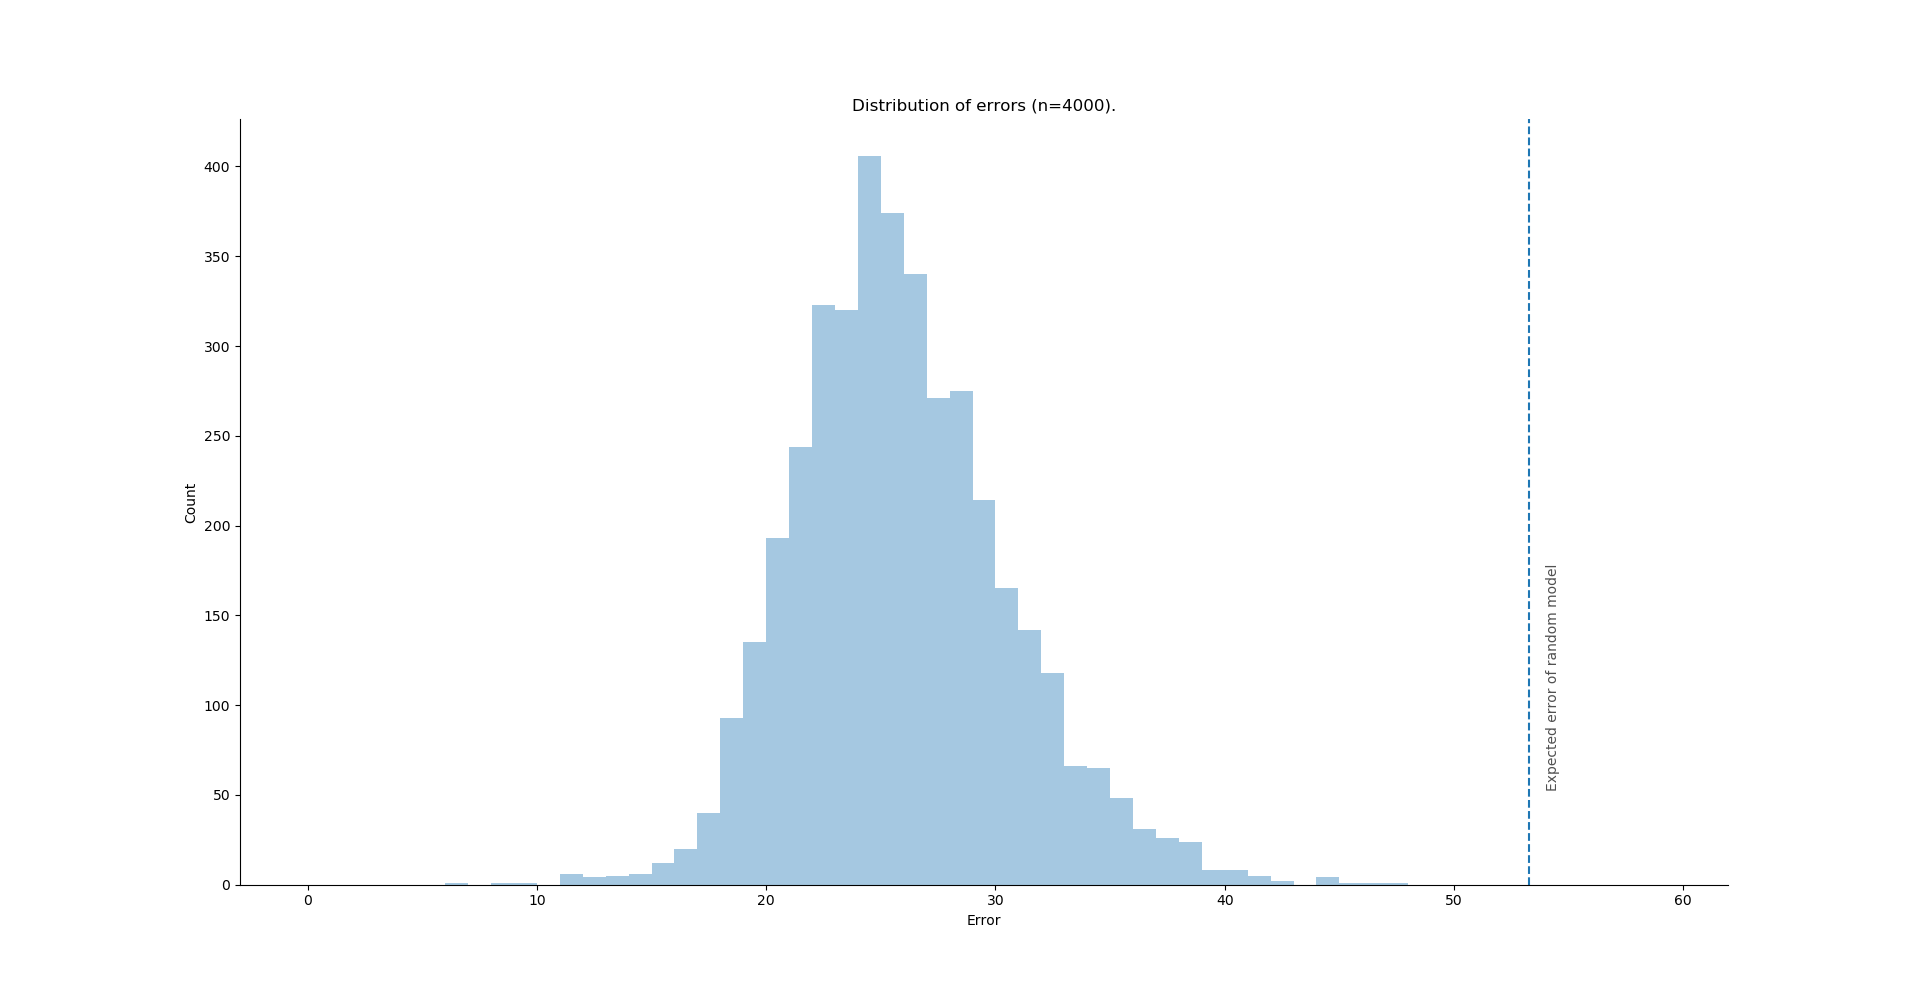
\includegraphics[width=\linewidth]{imgs_andy/error_distribution_200430m93s4000.png}
    \caption{Caption}
    \label{fig:error_dist}
\end{figure}

\begin{figure}
    \centering
    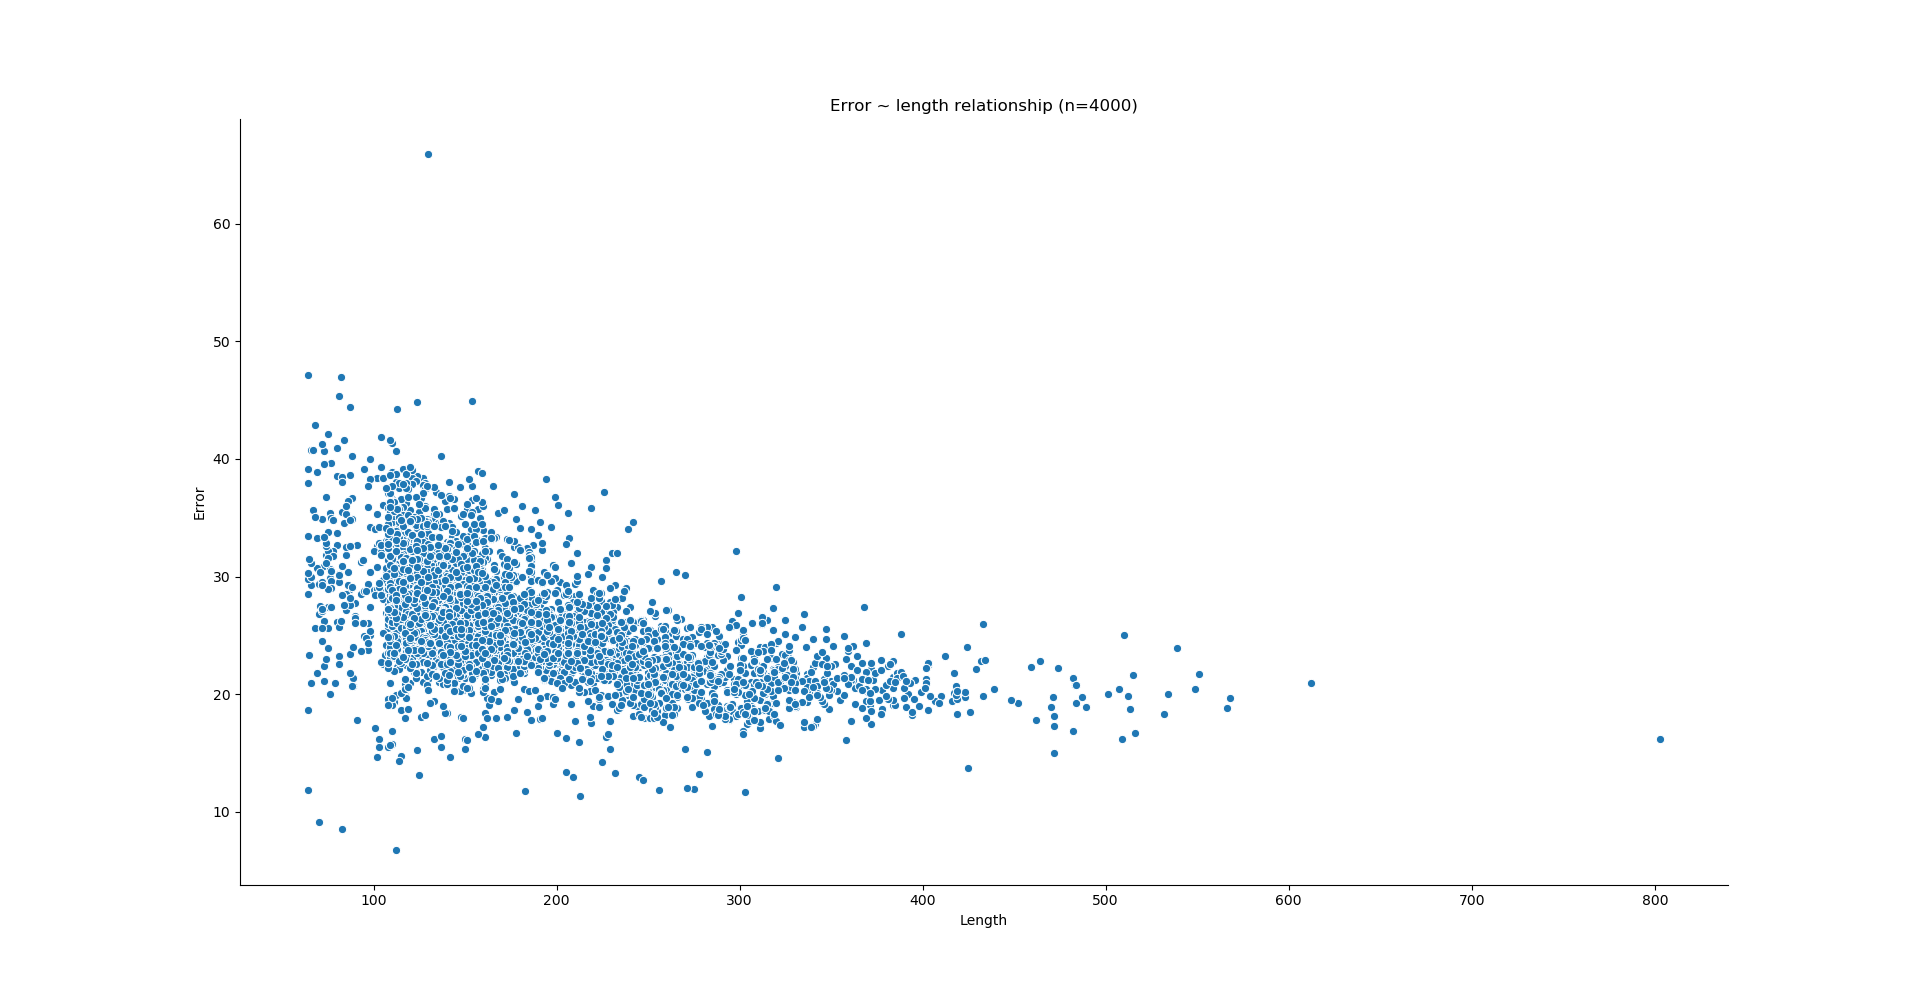
\includegraphics[width=\linewidth]{imgs_andy/error_length_200430m93s4000.png}
    \caption{Error - length relationship}
    \label{fig:err_len}
\end{figure}

\begin{figure}
    \centering
    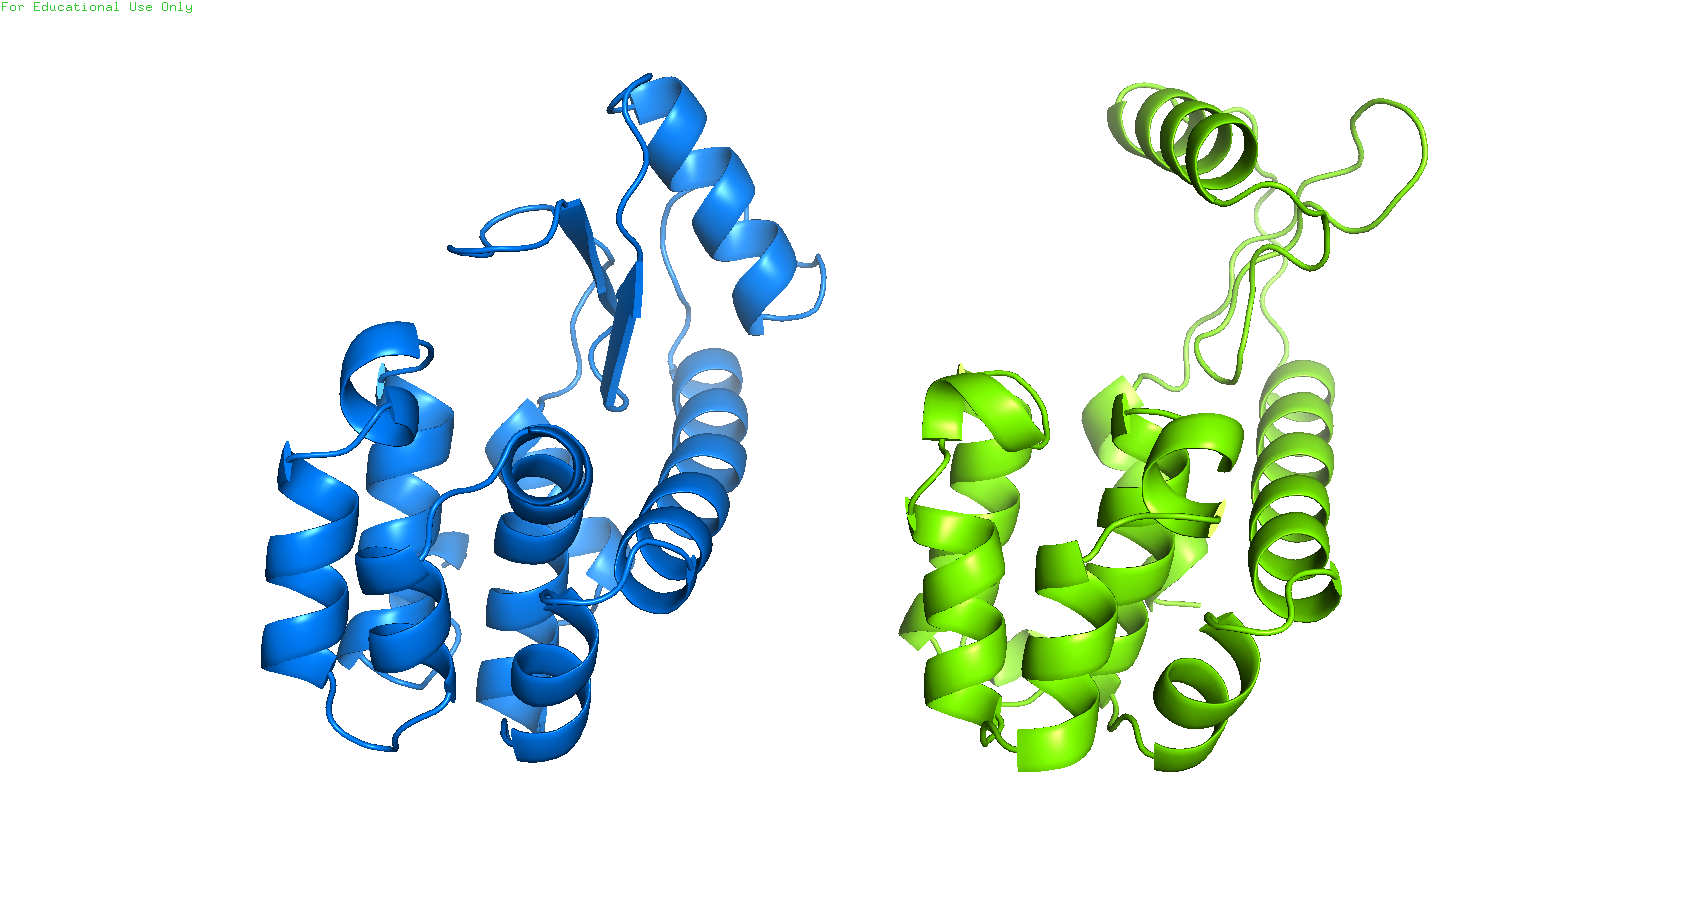
\includegraphics[width=\linewidth]{imgs_andy/139lA00_real_pred_3D_v2.png}
    \caption{Comparison of real vs. predicted 3D structure}
    \label{fig:real_pred}
\end{figure}

\begin{figure}
    \centering
    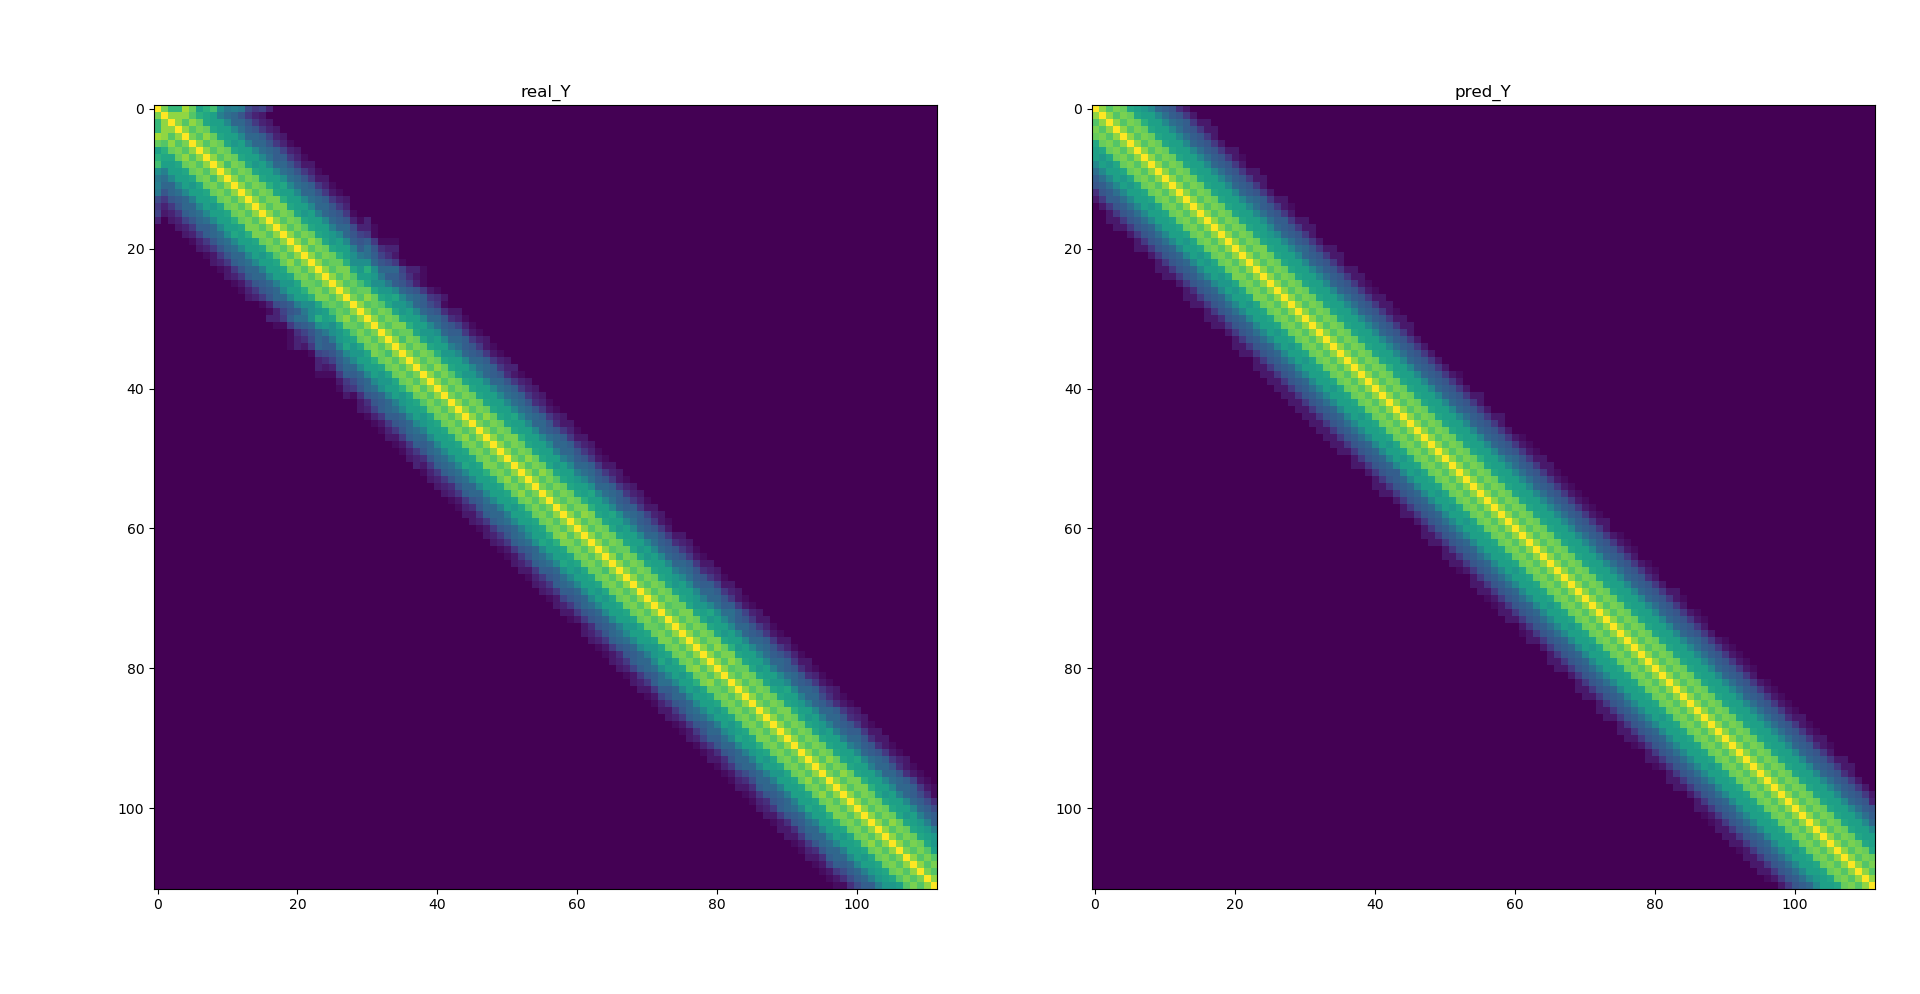
\includegraphics[width=\linewidth]{imgs_andy/2fxmB00_best_prediction.png}
    \caption{Best prediction}
    \label{fig:best}
\end{figure}

\begin{figure}
    \centering
    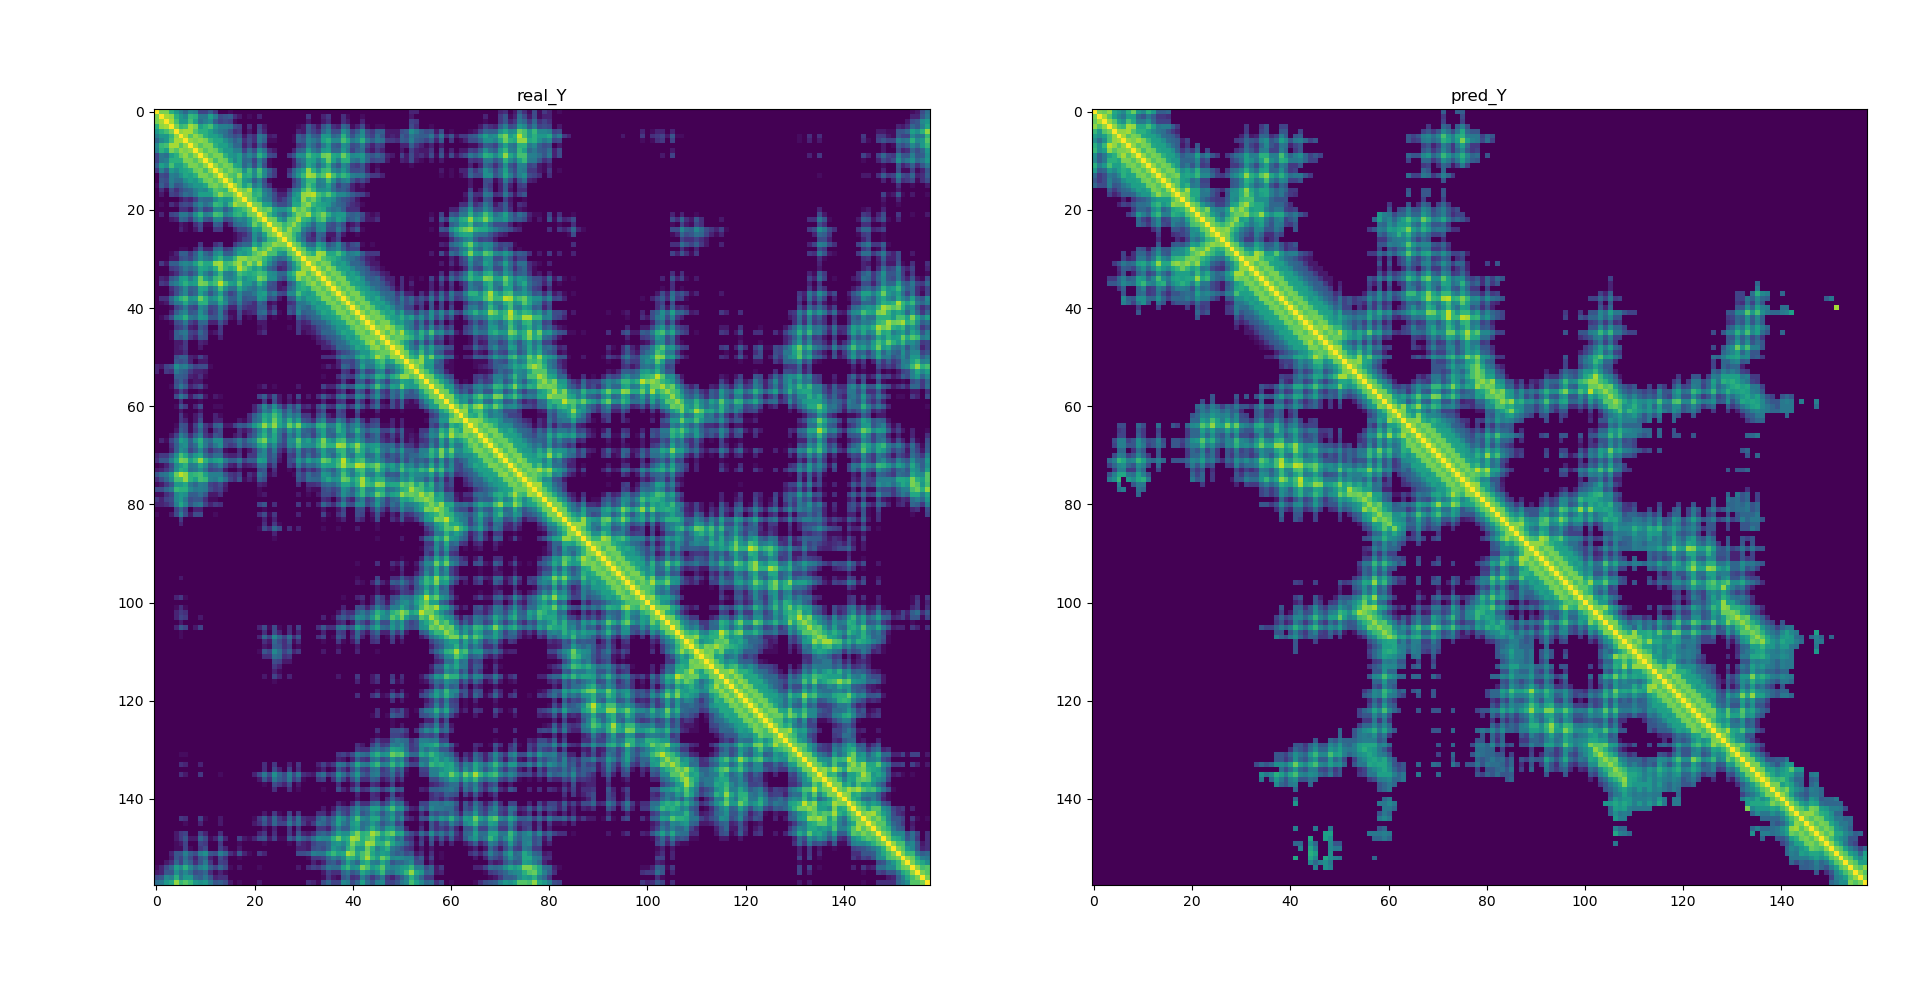
\includegraphics[width=\linewidth]{imgs_andy/1mdbA01_median_prediction.png}
    \caption{Median prediction}
    \label{fig:median}
\end{figure}

\begin{figure}
    \centering
    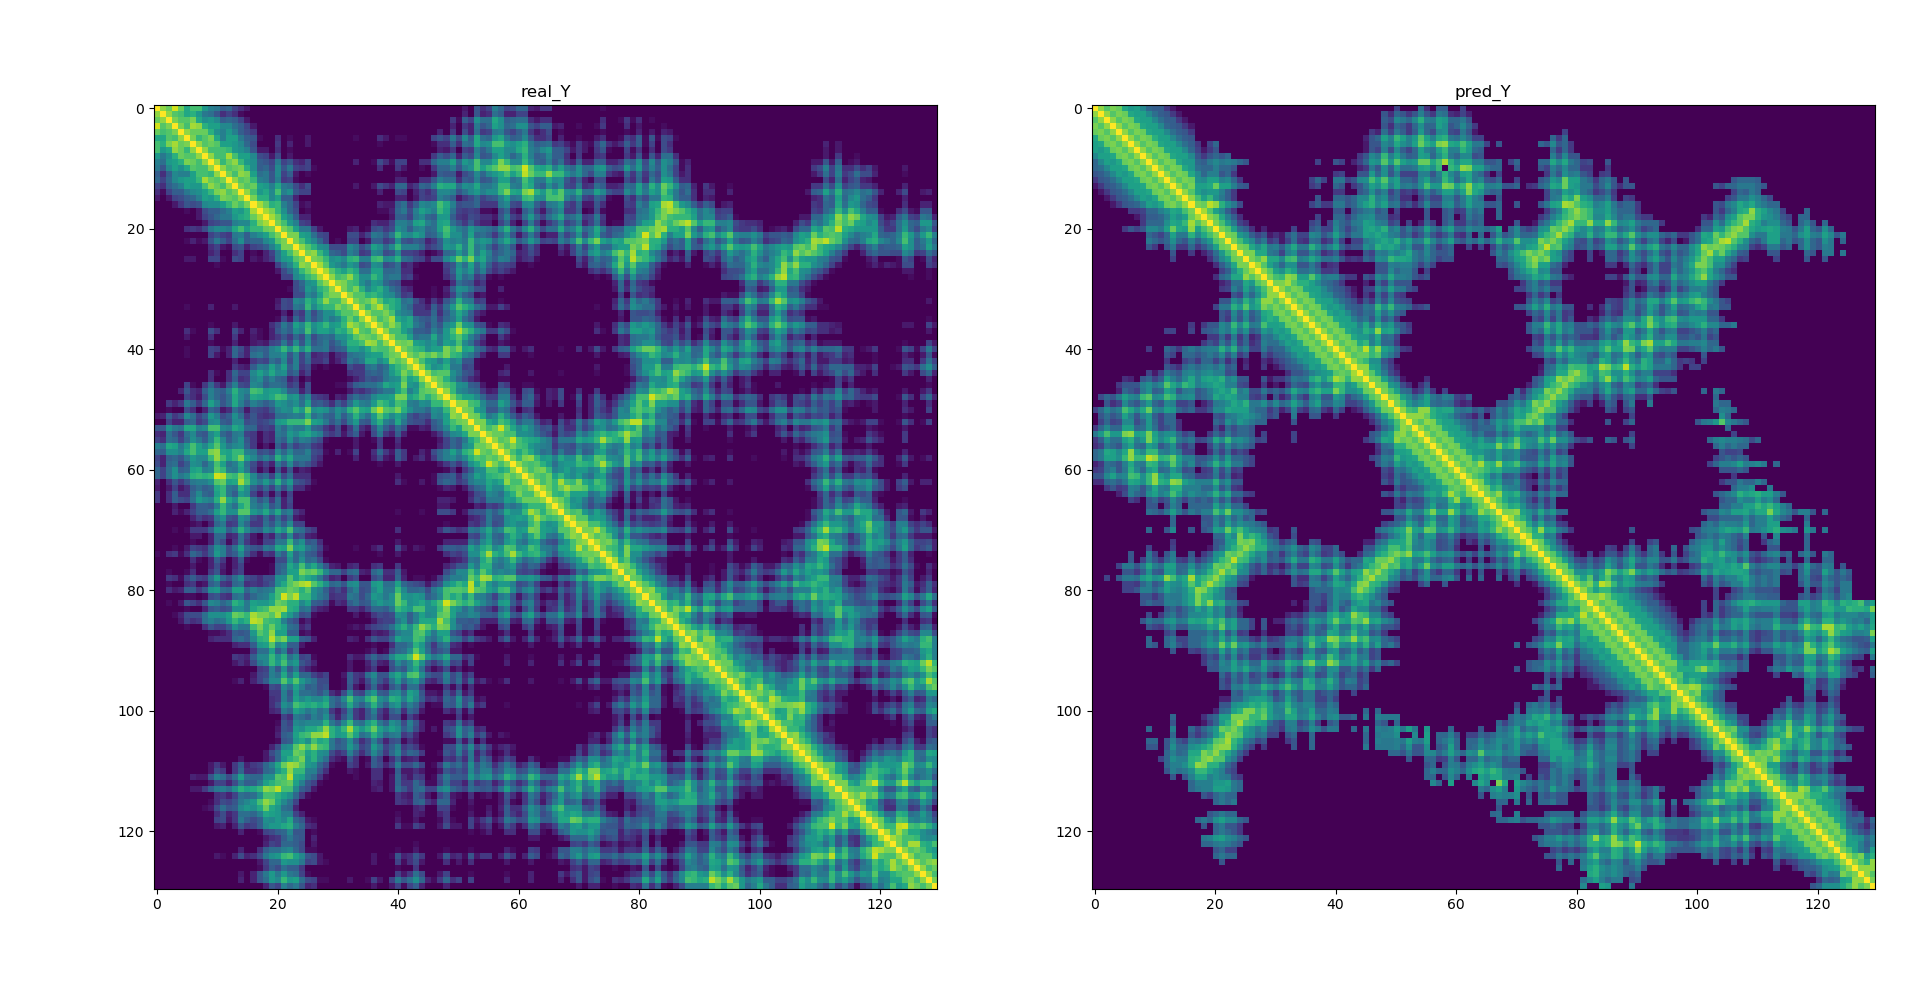
\includegraphics[width=\linewidth]{imgs_andy/3kitJ00_worst_prediction.png}
    \caption{Worst prediction}
    \label{fig:worst}
\end{figure}

\section{Structure Realization}

\section{Comparison with other methods}
\subsection{Distances}
\subsection{Structures}
